\documentclass[10pt,a4paper]{article}
\usepackage{amsmath}
\usepackage{graphicx}
\usepackage{hyperref}
\usepackage{caption}
\usepackage{subcaption}
\usepackage{listings}
\usepackage{xcolor}
\setlength\parindent{0pt}
\setlength{\parskip}{1em}

%%%%%%%%%%%%%%%%%%%%%%%%%%%
% MODIFY:

\newcommand{\authorA}{Qingyu Wang (03792094)}
\newcommand{\authorB}{Augustin Gaspard Camille Curinier (03784531)}
\newcommand{\authorC}{Yuxuan Wang  (03767260)}
\newcommand{\authorD}{Shihong Zhang (03764740)}
\newcommand{\authorE}{Mengshuo Li  (03792428)}
\newcommand{\groupNumber}{F} % - YOUR GROUP NUMBER
\newcommand{\exerciseNumber}{6} % - THE NUMBER OF THE EXERCISE

\newcommand{\workPerAuthor}{
\authorA & Task 1&20\%\\
      &Task 2&20\%\\
      &Task 3&20\%\\
      &Task 4&20\%\\
      &Task 5&20\%\\
      \hline
\authorB & Task 1&20\%\\
      &Task 2&20\%\\
      &Task 3&20\%\\
            &Task 4&20\%\\
      &Task 5&20\%\\
      \hline
\authorC & Task 1&20\%\\
      &Task 2&20\%\\
      &Task 3&20\%\\
            &Task 4&20\%\\
      &Task 5&20\%\\
      \hline
\authorD & Task 1&20\%\\
      &Task 2&20\%\\
      &Task 3&20\%\\
            &Task 4&20\%\\
      &Task 5&20\%\\
      \hline
\authorE & Task 1&20\%\\
      &Task 2&20\%\\
      &Task 3&20\%\\
      &Task 4&20\%\\
      &Task 5&20\%\\
}

%%%%%%%%%%%%%%%%%%%%%%%%%%%

\input{./imports.tex}

\begin{document}

\frontpage

\begin{task}{1,  Theoretical Analysis of the forward diffusion process in DDPM}
\section{Theoretical Analysis of the forward diffusion process in DDPM}
\subsection{Introduction}

Denoising Diffusion Probabilistic Models (DDPM) are advanced generative models that create high-quality data samples through a reverse noise diffusion process. A key step in these models is the forward diffusion process, which gradually transforms data samples into noise, laying the foundation for the denoising reverse process. This report aims to explain in detail the principles, mathematical derivation, and application of the forward diffusion process in DDPM.

\subsection{Overview of the Forward Diffusion Process}

The forward diffusion process progressively adds Gaussian noise to an initial data sample until it approximates pure noise. Given an initial data sample \( x_0 \), each step of this process can be viewed as a Markov chain, where the noise added at each step depends only on the previous step's result. This process is implemented through a series of conditional Gaussian distributions, ultimately "diffusing" the data sample into noise.

\subsection{Mathematical Definition}

The forward diffusion process for each step is defined by the following conditional distribution:

\[
q(x_t | x_{t-1}) = \mathcal{N}(x_t; \sqrt{\alpha_t} x_{t-1}, (1 - \alpha_t) I)
\]

where \(\alpha_t\) is a parameter controlling the noise level at each step, typically within (0, 1). To intuitively represent the noise level, we define \(\beta_t\) as:

\[
\beta_t = 1 - \alpha_t
\]

Thus, the conditional distribution can be rewritten as:

\[
q(x_t | x_{t-1}) = \mathcal{N}(x_t; \sqrt{1 - \beta_t} x_{t-1}, \beta_t I)
\]

\subsection{Mathematical Derivation}

\subsection*{Deriving the Distribution from \( x_0 \) to \( x_t \)}

To derive the distribution from the initial sample \( x_0 \) to any timestep \( t \), \( q(x_t | x_0) \), we use the Markov property, expressing the process as:

\[
q(x_t | x_0) = \int q(x_t | x_{t-1}) q(x_{t-1} | x_{t-2}) \cdots q(x_1 | x_0) \, dx_{t-1} \cdots dx_1
\]

Since each step is a linear transformation of Gaussian distributions, the result is also a Gaussian distribution. Using mathematical induction, we obtain:

\[
q(x_t | x_0) = \mathcal{N}(x_t; \sqrt{\bar{\alpha}_t} x_0, (1 - \bar{\alpha}_t) I)
\]

where:

\[
\bar{\alpha}_t = \prod_{s=1}^t \alpha_s
\]

We define the cumulative noise parameter as:

\[
\bar{\beta}_t = 1 - \bar{\alpha}_t
\]

Thus, any step \( x_t \) in the forward diffusion process can be expressed as:

\[
x_t = \sqrt{\bar{\alpha}_t} x_0 + \sqrt{1 - \bar{\alpha}_t} \epsilon
\]

where \(\epsilon \sim \mathcal{N}(0, I)\) is standard normal noise.

\subsection{Application and Significance}

The key to the forward diffusion process lies in its foundation for the reverse denoising process. In DDPM, the model's training objective is to learn how to recover high-quality data from noise samples through a reverse process. The forward process provides the mapping from data to noise, enabling the model to perform symmetric denoising.

\end{task}
\newpage

\begin{task}{2,  Theoretical Analysis of the reverse diffusion process in DDPM}
\section{ Theoretical Analysis of the reverse diffusion process in DDPM}
\subsection{Introduction}

Denoising Diffusion Probabilistic Models (DDPM) are a class of generative models that excel in generating high-quality data samples, particularly in image generation tasks. The forward diffusion process gradually corrupts data with Gaussian noise, transforming it into a near-pure noise state. The reverse diffusion process, which is the focus of this report, aims to revert this noisy data back to the original high-quality samples. This report provides an in-depth explanation of the principles, mathematical derivation, and application of the reverse diffusion process in DDPM.

\subsection{Overview of the Reverse Diffusion Process}

The reverse diffusion process is the cornerstone of DDPM. It involves learning to reverse the noise added during the forward diffusion process. Given a noisy sample \( x_T \) (where \( T \) denotes the final timestep in the forward process), the goal is to progressively denoise this sample to recover the original data \( x_0 \). This process is achieved through a series of learned reverse transitions.

\subsection{Mathematical Definition}

The reverse diffusion process is defined by a series of learned conditional distributions that approximate the reverse transitions of the forward diffusion process. Specifically, the reverse process can be formulated as:

\[
p_\theta(x_{t-1} | x_t) = \mathcal{N}(x_{t-1}; \mu_\theta(x_t, t), \Sigma_\theta(x_t, t))
\]

Here, \( \mu_\theta \) and \( \Sigma_\theta \) are the mean and variance predicted by a neural network parameterized by \( \theta \). These parameters are learned to closely approximate the true reverse transition distributions.

\subsection{Mathematical Derivation}

\subsection*{Deriving the Reverse Conditional Distributions}

The forward diffusion process is defined by:

\[
q(x_t | x_{t-1}) = \mathcal{N}(x_t; \sqrt{1 - \beta_t} x_{t-1}, \beta_t I)
\]

where \( \beta_t = 1 - \alpha_t \). Using the property of Gaussian distributions, we can derive the form of the reverse conditional distributions:

\[
q(x_{t-1} | x_t, x_0) \propto q(x_t | x_{t-1}) q(x_{t-1} | x_0)
\]

Since both \( q(x_t | x_{t-1}) \) and \( q(x_{t-1} | x_0) \) are Gaussians, the product of Gaussians is also Gaussian. This allows us to write:

\[
q(x_{t-1} | x_t, x_0) = \mathcal{N}(x_{t-1}; \tilde{\mu}_t(x_t, x_0), \tilde{\beta}_t I)
\]

where \( \tilde{\mu}_t(x_t, x_0) \) and \( \tilde{\beta}_t \) can be derived through standard Gaussian manipulation techniques. For simplicity, the approximations used in DDPM lead to:

\[
\tilde{\mu}_t(x_t, x_0) = \frac{\sqrt{\bar{\alpha}_{t-1}} \beta_t}{1 - \bar{\alpha}_t} x_0 + \frac{\sqrt{\alpha_t}(1 - \bar{\alpha}_{t-1})}{1 - \bar{\alpha}_t} x_t
\]

and

\[
\tilde{\beta}_t = \frac{1 - \bar{\alpha}_{t-1}}{1 - \bar{\alpha}_t} \beta_t
\]

\subsection*{Parameterization and Learning}

The parameterization and learning process in Denoising Diffusion Probabilistic Models (DDPMs) begins with the goal of maximizing the log-likelihood of the data. The log-likelihood estimation provides a measure of how well the model explains the observed data. Formally, the log-likelihood can be expressed as:

\[
\log p_\theta(x_0)
\]

However, directly maximizing this log-likelihood is intractable due to the complex dependencies between the data points. Therefore, an alternative approach is employed by introducing a variational distribution \( q \) to approximate the true posterior distribution.

To make the optimization tractable, the problem is reformulated into maximizing the Evidence Lower Bound (ELBO). The ELBO serves as a lower bound to the log-likelihood and is easier to optimize. The ELBO can be derived as follows:

\[
\log p_\theta(x_0) \geq \mathbb{E}_{q(x_{1:T} | x_0)} \left[ \log p_\theta(x_0 | x_{1:T}) \right] - \text{KL}(q(x_{1:T} | x_0) \| p_\theta(x_{1:T}))
\]

This reformulation decomposes the log-likelihood into the reconstruction error and KL divergence terms.

\begin{itemize}
    \item \textbf{Reconstruction Error Term}:
    \[
    \mathbb{E}_{q(x_{1:T} | x_0)} \left[ \log p_\theta(x_0 | x_{1:T}) \right]
    \]
    This term measures how well the model reconstructs the original data \( x_0 \) from the noisy data \( x_{1:T} \).

    \item \textbf{KL Divergence Term}:
    \[
    \sum_{t=1}^T \mathbb{E}_{q(x_{t-1} | x_t, x_0)} \left[ \text{KL}(q(x_t | x_{t-1}) \| p_\theta(x_t | x_{t-1})) \right]
    \]
    This term measures the divergence between the true forward process \( q \) and the learned reverse process \( p_\theta \).
\end{itemize}

Based on empirical findings, it is often sufficient to focus on the mean while ignoring the variance in the KL divergence term. This simplification reduces computational complexity and still achieves good performance. The mean is crucial for capturing the primary structure of the data, while the variance, although important, can be approximated or even ignored in certain scenarios.

By simplifying the KL divergence to primarily consider the mean, the ELBO can be further streamlined. This approach leverages the fact that the mean often captures the most significant aspects of the data distribution, making it a practical choice for efficient learning.

Through these simplifications, the final equations for the parameterization and learning in DDPMs are derived. The neural network predicts the noise \( \epsilon_\theta(x_t, t) \) added during the forward process, and the mean \( \mu_\theta \) is adjusted accordingly. The resulting prediction for \( x_{t-1} \) is given by:

\[
x_{t-1} = \frac{1}{\sqrt{\alpha_t}} \left( x_t - \frac{1 - \alpha_t}{\sqrt{1 - \bar{\alpha}_t}} \epsilon_\theta(x_t, t) \right) + \sqrt{\beta_t} z_t
\]

where \( z_t \sim \mathcal{N}(0, I) \) is sampled noise.

\subsection{Training Objective}

The training objective for DDPM involves minimizing the difference between the true noise \( \epsilon \) and the predicted noise \( \epsilon_\theta \). This is typically done using a simple mean squared error (MSE) loss:

\[
\mathcal{L}(\theta) = \mathbb{E}_{x_0, \epsilon, t} \left[ \left\| \epsilon - \epsilon_\theta(x_t, t) \right\|^2 \right]
\]

where \( x_t = \sqrt{\bar{\alpha}_t} x_0 + \sqrt{1 - \bar{\alpha}_t} \epsilon \).

\subsection{Application and Significance}

The reverse diffusion process is crucial for the practical application of DDPMs. By effectively learning to denoise a progressively corrupted sample, the model can generate high-quality samples from pure noise. This approach has demonstrated impressive results in various data generation tasks, including image synthesis and audio generation.


\end{task}


\newpage
\begin{task}{3, Code Replication Task}
\section{Code Replication Task}
The code is divided into two main functions: \texttt{train} and \texttt{eval}, each with several key steps. The \texttt{train} function is responsible for setting up the dataset, model, optimizer, and training loop. The \texttt{eval} function is used to evaluate the model by generating images from noise and saving them. Here is a detailed explanation in a structured format.

\subsection{Importing Modules}

\begin{itemize}
    \item \textbf{Configuration and Directories:} The script sets the batch size, number of epochs, learning rate, and warmup epochs. It also creates an output directory to save model checkpoints and sampled images.
    \item \textbf{Data Transformations and Dataset: } The CIFAR-10 dataset is loaded with transformations including normalization.
    \item \textbf{Model and Optimizer:} A UNet model is initialized and moved to GPU. An Adam optimizer is set up with the specified learning rate.
    \item \textbf{Scheduler:} A gradual warmup scheduler is defined to gradually increase the learning rate for the first few epochs, followed by a step LR scheduler.
    \item \textbf{Gaussian Diffusion Trainer:} The GaussianDiffusionTrainer is initialized.
    \item \textbf{Training Loop:} For each epoch, the model is trained, and the loss is logged. Every 10 epochs, sampled images are generated and saved. Model checkpoints are saved at the end of each epoch.
\end{itemize} 

These imports include necessary libraries for data handling, model building, training, and evaluation.

\subsection{Train Function}

\subsubsection{Setup Device and Dataset}

This code defines a \texttt{‘train’} function that takes a dictionary \texttt{‘modelConfig’} containing training configurations as an argument. First, it sets up the computing device (either CPU or GPU) based on the value in \texttt{‘modelConfig["device"]’}. Then, it loads the CIFAR-10 training dataset and applies a series of data augmentation and preprocessing operations. These operations include randomly flipping the images horizontally, converting the images to PyTorch tensors, and normalizing the images so that their pixel values have a mean and standard deviation of 0.5. These preprocessing steps help improve the model's generalization capabilities.

Next, the code creates a \texttt{'DataLoader'} to iterate over the dataset in mini-batches. The \texttt{'DataLoade'r} is configured with the following parameters: batch size obtained from \texttt{'modelConfig["batch-size"]'}, shuffling the data at each epoch, using 4 subprocesses to load the data in parallel, dropping the last incomplete batch if the dataset size is not divisible by the batch size, and pinning memory to speed up data transfer to the GPU. These steps ensure that the data is efficiently loaded and preprocessed during training, providing a solid foundation for training the model.

\subsubsection{Model Initialization and Optimizer Setup}

\begin{itemize}
    \item \textbf{Model Initialization:} Initializes the UNet model with parameters from modelConfig and moves it to the specified device.
    \item \textbf{Loading Pre-trained Weights:} If specified, loads pre-trained weights into the model.
    \item \textbf{Optimizer:} Sets up the AdamW optimizer with a specified learning rate and weight decay.
    \item \textbf{Learning Rate Scheduler:} Configures a cosine annealing learning rate scheduler and a warmup scheduler to gradually increase the learning rate at the start of training.
    \item \textbf{Trainer Initialization:} Sets up a Gaussian diffusion trainer with the initialized model and diffusion parameters, moving it to the specified device.
\end{itemize}
   

\subsubsection{Training Loop}

\begin{itemize}
    \item \textbf{Training Loop:}
The training process iterates through a number of epochs specified by \texttt{modelConfig["epoch"]}. This outer loop controls how many times the model will see the entire dataset during training. Each epoch represents one full pass over the entire training data.

\item \textbf{Data Loading and Progress Bar}
For each epoch, the code wraps the \texttt{dataloader} with a \texttt{tqdm} progress bar, providing a dynamic and informative console output that tracks the training progress in real-time. This allows the user to monitor the current state of the training process, including the number of batches processed, the speed of processing, and other relevant metrics.

\item \textbf{Mini-batch Training}
Within each epoch, the model trains on mini-batches of data. For each mini-batch, the gradients are reset using \texttt{optimizer.zero\_grad()}. The images are transferred to the specified computing device (\texttt{x\_0 = images.to(device)}), and the loss is computed using the \texttt{trainer} and scaled down (\texttt{loss = trainer(x\_0).sum() / 1000.}). Backpropagation is then performed to compute the gradients (\texttt{loss.backward()}), and the gradients are clipped to prevent them from exploding (\texttt{torch.nn.utils.\\clip\_grad\_norm\_(net\_model.parameters(), modelConfig["grad\_clip"])}). Finally, the model parameters are updated based on the computed gradients (\texttt{optimizer.step()}).

\item \textbf{Progress Bar Updates}
Throughout the mini-batch training, the progress bar is continuously updated with key metrics. These include the current epoch number, the loss value, the shape of the input images, and the current learning rate. This provides a clear and concise overview of the training status, helping to track the model's performance and the training process's progression.

\item \textbf{Learning Rate Scheduling}
At the end of each epoch, the learning rate is adjusted using the warm-up scheduler (\texttt{warmUpScheduler.step()}). This scheduler initially increases the learning rate gradually (warm-up phase) and then adjusts it according to a cosine annealing schedule. This approach helps to stabilize training, allowing the model to converge more effectively.

\item \textbf{Checkpoint Saving}
After completing the mini-batch training for an epoch, the model's state dictionary (containing its parameters) is saved to a specified directory (\texttt{modelConfig["save\_weight\_dir"]}). The checkpoint filenames include the current epoch number, ensuring that model states are saved incrementally (\texttt{'ckpt\_\ ' + str(e) + "\_.pt"}). This allows for model recovery and continued training from specific points, providing a safeguard against potential interruptions and enabling more flexible training management.
\end{itemize}
   

\subsection{Eval Function}

\subsubsection{Model Loading and Evaluation Setup}
The \texttt{eval} function is designed to evaluate a pre-trained UNet model based on the configuration specified in the \texttt{modelConfig} dictionary. The function performs the following steps:

\begin{itemize}
    \item \textbf{Disable Gradient Calculation}: The function uses \texttt{torch.no\_grad()} to disable gradient calculations, which reduces memory consumption and speeds up computations during evaluation.
    
    \item \textbf{Device Configuration}: It sets up the computing device (CPU or GPU) using \texttt{modelConfig["device"]}.
    
    \item \textbf{Model Initialization}: The function initializes a UNet model with parameters from \texttt{modelConfig} such as the number of timesteps (\texttt{T}), the number of input channels (\texttt{ch}), channel multiplier (\texttt{ch\_mult}), attention mechanism (\texttt{attn}), and the number of residual blocks (\texttt{num\_res\_blocks}). Dropout is set to 0 for evaluation.
    
    \item \textbf{Load Pre-trained Weights}: It loads the pre-trained model weights from a specified path (\texttt{modelConfig\newline["save\_weight\_dir"]} and \texttt{modelConfig["test\_load\_weight"]}) and applies these weights to the model using \texttt{model.load\_state\_dict(ckpt)}.
    
    \item \textbf{Set Model to Evaluation Mode}: The model is switched to evaluation mode using \texttt{model.eval()}, which affects certain layers like dropout and batch normalization to behave appropriately during evaluation.
    
    \item \textbf{Initialize Sampler}: A \texttt{GaussianDiffusionSampler} is instantiated with the model and diffusion process parameters (\texttt{beta\_1}, \texttt{beta\_T}, \texttt{T}), and moved to the specified device.
\end{itemize}

By following these steps, the function prepares the UNet model for inference or sampling using a Gaussian diffusion process, ensuring that the model operates correctly and efficiently in an evaluation context.
\subsubsection{Image Sampling and Saving}


\begin{itemize}
    \item \textbf{Generate Noisy Image}: 
    A noisy image tensor is generated using \texttt{torch.randn}, with dimensions \texttt{[modelConfig["batch\_size"], 3, 32, 32]}, and allocated to the specified device (\texttt{device}). This tensor represents a batch of noisy images with 3 color channels and a resolution of 32x32 pixels.

    \item \textbf{Clamp and Save Noisy Image}: 
    The noisy images are scaled and clamped to the range [0, 1] using \texttt{torch.clamp} and a linear transformation. This ensures the pixel values are suitable for image display. The processed noisy images are saved to the directory specified in \texttt{modelConfig["sampled\_dir"]} with the filename provided in \texttt{modelConfig["sampledNoisyImgName"]}. The images are saved in a grid with a specified number of rows (\texttt{nrow}).

    \item \textbf{Sample Images from Model}: 
    The noisy images are passed through a pre-trained sampler (e.g., a diffusion model) to generate sampled images. The sampled images are scaled to the range [0, 1] using a similar linear transformation to make them suitable for display.

    \item \textbf{Save Sampled Images}: 
    The sampled images are saved to the directory specified in \texttt{modelConfig\newline["sampled\_dir"]} with the filename provided in \texttt{modelConfig["sampledImgName"]}. The images are saved in a grid with the specified number of rows (\texttt{nrow}).
\end{itemize}
\subsection{Inference and Training Process Analysis}

\subsubsection{Inference Process Description}

The inference process involves loading the trained model, setting up the sampler, and generating images from noise. Below is a detailed description of each step.

\textbf{1. Model Loading and Evaluation Setup}

\begin{itemize}
    \item \textbf{Disable Gradient Calculation}: Gradient calculation is disabled to save memory and improve performance during inference.
    \item \textbf{Device Configuration}: The device (CPU or GPU) is set based on the provided configuration.
    \item \textbf{Model Initialization}: A U-Net model is initialized with parameters specified in the configuration.
    \item \textbf{Loading Pre-trained Weights}: The pre-trained weights are loaded into the model.
    \item \textbf{Model Evaluation Mode}: The model is set to evaluation mode to disable dropout and batch normalization updates.
    \item \textbf{Sampler Initialization}: A Gaussian diffusion sampler is initialized with the model and diffusion parameters.
\end{itemize}

\textbf{2. Image Sampling and Saving}

\begin{itemize}
    \item \textbf{Noise Image Generation}: A batch of noisy images is sampled from a standard normal distribution.
    \item \textbf{Save Noisy Images}: The noisy images are scaled to the [0, 1] range and saved.
    \item \textbf{Image Generation}: The sampler generates images from the noisy images using the reverse diffusion process.
    \item \textbf{Save Generated Images}: The generated images are scaled to the [0, 1] range and saved.
\end{itemize}

\subsubsection{Training Process Description}

The training process involves several key steps, including setting up the device and dataset, initializing the model and optimizer, and running the training loop. Below is a detailed description of each step.

\textbf{1. Setup Device and Dataset}

\begin{itemize}
    \item \textbf{Device Configuration}: The device (CPU or GPU) is set based on the provided configuration.
    \item \textbf{Dataset Loading}: The CIFAR-10 dataset is loaded with specific transformations:
    \begin{itemize}
        \item Random horizontal flip for data augmentation.
        \item Conversion to tensor format.
        \item Normalization to have a mean of 0.5 and a standard deviation of 0.5 for each channel.
    \end{itemize}
    \item \textbf{DataLoader}: A DataLoader is created to iterate over the dataset in batches, with shuffling and multi-threaded data loading.
\end{itemize}

\textbf{2. Model Initialization and Optimizer Setup}

\begin{itemize}
    \item \textbf{Model Setup}: A U-Net model is initialized with parameters specified in the configuration.
    \item \textbf{Loading Pre-trained Weights}: If pre-trained weights are provided, they are loaded into the model.
    \item \textbf{Optimizer Configuration}: The AdamW optimizer is configured with a specified learning rate and weight decay.
    \item \textbf{Learning Rate Schedulers}: Two schedulers are set up:
    \begin{itemize}
        \item \textbf{CosineAnnealingLR}: For cosine annealing with a minimum learning rate.
        \item \textbf{GradualWarmupScheduler}: To gradually warm up the learning rate for a fraction of the total epochs, followed by cosine annealing.
    \end{itemize}
    \item \textbf{Diffusion Trainer}: A Gaussian diffusion trainer is initialized with the model and diffusion parameters.
\end{itemize}

\textbf{3. Training Loop}

\begin{itemize}
    \item \textbf{Epoch Iteration}: The training loop iterates over the specified number of epochs.
    \item \textbf{Batch Processing}: For each batch of data:
    \begin{itemize}
        \item Gradients are reset to zero.
        \item Images are moved to the device.
        \item Loss is computed using the diffusion trainer.
        \item Backpropagation is performed to compute gradients.
        \item Gradients are clipped to prevent exploding gradients.
        \item Model parameters are updated using the optimizer.
        \item Training progress is displayed using \texttt{tqdm}.
    \end{itemize}
    \item \textbf{Scheduler Step}: The warm-up scheduler is updated after each epoch.
    \item \textbf{Model Checkpointing}: Model weights are saved at the end of each epoch.
\end{itemize}
\subsection{Summary}

\begin{itemize}
    \item \textbf{Importing Modules}: Import required libraries and custom modules.
    \item \textbf{Train Function}:
        \begin{itemize}
            \item \textbf{Setup Device and Dataset}: Initialize the device and load the CIFAR-10 dataset with transformations.
            \item \textbf{Model Initialization and Optimizer Setup}: Initialize the U-Net model, optimizer, and learning rate schedulers. Load pre-trained weights if available.
            \item \textbf{Training Loop}: Iterate over epochs and batches, compute loss, perform backpropagation, update model parameters, and save model weights.
        \end{itemize}
    \item \textbf{Eval Function}:
        \begin{itemize}
            \item \textbf{Model Loading and Evaluation Setup}: Load the model weights, set up the model for evaluation, and initialize the sampler.
            \item \textbf{Image Sampling and Saving}: Generate images from noise, scale them, and save the noisy and sampled images.
        \end{itemize}
\end{itemize}
\end{task}



\newpage
\begin{task}{4, Training Task}
\section{Training Task}
Through the training process, we obtained results with Epoch values equal to 0, 50, 100, 150, and 199, respectively. The result is shown below. 
\begin{figure}[H]
    \centering
    \includegraphics[width=0.8\textwidth]{0.png}
    \caption{Epoch=0}
    \label{fig:training_process}
\end{figure}
\textbf{Initial State:} At the beginning of training, the images generated by the model are almost entirely noise, with no discernible objects or shapes. The model has not learned anything yet, and the generated images are indistinguishable from the input noise.

\begin{figure}[H]
    \centering
    \includegraphics[width=0.8\textwidth]{50.png}
    \caption{Epoch=50}
    \label{fig:training_process}
\end{figure}
\textbf{Early Training:} After 50 epochs of training, the generated images start to show some blurry shapes and colors, but still lack clear structure or objects.The model is beginning to learn some basic features of the data, but more training is needed to improve the quality of the generated images.
\begin{figure}[H]
    \centering
    \includegraphics[width=0.8\textwidth]{100.png}
    \caption{Epoch=100}
    \label{fig:training_process}
\end{figure}
\textbf{Mid Training:} After 100 epochs, the generated images start to show more distinct shapes and objects, though there is still noticeable blurriness and distortion.The model has learned more features of the data, and the quality of the generated images has improved, but further training is required to produce clearer images.
\begin{figure}[H]
    \centering
    \includegraphics[width=0.8\textwidth]{150.png}
    \caption{Epoch=150}
    \label{fig:training_process}
\end{figure}
\textbf{Late Training:} After 150 epochs, the generated images become clearer, with more discernible details in the shapes and objects.The model has continued to improve during training and is now capable of generating fairly clear and realistic images, though some details still need refinement.
\begin{figure}[H]
    \centering
    \includegraphics[width=0.8\textwidth]{199.png}
    \caption{Epoch=199}
    \label{fig:training_process}
\end{figure}
\textbf{Final State:} After 199 epochs, the quality of the generated images has further improved, with more precise details and overall image quality approaching that of real images.After sufficient training, the model can generate high-quality images, nearly achieving the desired level of realism.

From these images at different epoch values, we can see that the quality of the generated images gradually improves with increased training. The model starts from complete noise, gradually learning the features of the data, and eventually producing clearer and more realistic images. This indicates that the model continuously improves during training, eventually mastering the ability to generate high-quality images.

\end{task}



\newpage
\begin{task}{5, Training the model on pedestrians data}
\section{Training the model on pedestrians data}
\subsection{Introduction}
The Diffusion Probabilistic Model (DDPM) is a generative model capable of producing high-quality samples by learning the distribution of a dataset through a process of adding and removing noise. In this project, we implement a DDPM to generate pedestrian trajectories. The model is trained on a dataset of pedestrian positions and is designed to learn the underlying patterns of these trajectories over time. This report provides a detailed overview of the model architecture, training procedure, sampling process, and results.
\subsection{Task Description}
Each training sample in our dataset represents the positions of 100 pedestrians at a specific time step, which can be expressed as a 200-dimensional vector (2 coordinates per pedestrian). The dataset consists of multiple time steps, with each time step being represented by a separate 200-dimensional vector. Our objective is to train the DDPM to learn the distribution of these vectors so that it can generate realistic pedestrian positions at random time.
\subsection{Designing dataset}
First of all, we need to design the dataset consisting of the trajectories of 100 pedestrians over time for the training and recovering. 
\subsection*{Start and end point}
To make sure the dataset is large enough for training, we set the size of dataset to around 40000 steps. This number varies according to when all the pedestrians arrives the destination. We simulated the trajectory of 100 pedestrians in the MI building. The 100 pedestrians are divided into 5 groups, starting from different positions of MI building. Pedestrians from different groups arrive at their respective way points, and then arrive at the critical zone, finally leave the building. The start points, way points and end points are shown in the following figure.
\begin{figure}[h!]
    \centering
    \includegraphics[width=10cm,height=7cm]{waypoints.png}
    \caption{Start points, way points and end points}
    \label{fig:1}
\end{figure}

\subsection*{Generate the trajectories}
The pedestrians start from their start points, go through the way points and then arrive at the critical zone, finally leave the building. First of all, we calculate the direction of each pedestrian.
\begin{equation}
    Direction = target\_point - current\_position
\end{equation}

To make sure that their trajectories are different, we added a noise when generate their trajectories. In each time step, we can calculate the position of each pedestrian by following,
\begin{equation}
    New\_positions = current\_position + direction * step\_size + noise
\end{equation}

This allows us to generate the trajectories of 100 pedestrians and to ensure that their trajectories are different. The step size allows us to adjust the step number of the pedestrians. The following figure shows the positions of the pedestrians in different time steps.
\begin{figure}[h!]
    \centering
    \includegraphics[width=15cm,height=12cm]{timeseries.png}
    \caption{Positions of the pedestrians in different time steps}
    \label{fig:2}
\end{figure}
\end{task}

After simulating around 40000 steps, we can obtain the data set for training. The following figure shows the trajectories of 100 pedestrians.
\begin{figure}[h!]
    \centering
    \includegraphics[width=10cm,height=7cm]{tr.png}
    \caption{Positions of the pedestrians in different time steps}
    \label{fig:3}
\end{figure}

\newpage
\subsection{Model Architecture}
The core of our DDPM implementation is a 1D U-Net, which is particularly well-suited for processing sequential data such as pedestrian trajectories. The U-Net consists of an encoder and decoder, connected through skip connections that allow the model to capture both local and global patterns in the data.

\subsection*{UNet1D}

\begin{itemize}
    \item \textbf{Encoder}: The encoder compresses the input data into a lower-dimensional representation. It consists of several convolutional layers with ReLU activation functions and batch normalization.
    \item \textbf{Time Embedding}: Time steps are embedded using a sinusoidal embedding, allowing the model to incorporate temporal information.
    \item \textbf{Decoder}: The decoder reconstructs the data from the compressed representation, using transposed convolutional layers to upsample the data back to its original size.
    \item \textbf{Skip Connections}: Skip connections are used to pass information from the encoder layers directly to the corresponding decoder layers, preserving spatial information that might otherwise be lost during downsampling.
\end{itemize}

\subsection{Training Procedure}

The training process involves iteratively optimizing the model to minimize the reconstruction loss between the predicted and actual pedestrian positions. The steps are as follows:

\begin{enumerate}
    \item \textbf{Data Loading}: Load the dataset of pedestrian positions, normalize it to the range [0, 1], and reshape it to the required format.
    \item \textbf{Adding Noise}: At each training step, add Gaussian noise to the input data to create noisy samples.
    \item \textbf{Model Training}: Train the model to predict the original (non-noisy) data from the noisy samples. The model uses the Adam optimizer and Mean Squared Error (MSE) loss.
    \item \textbf{Checkpointing}: Periodically save the model's weights to allow for recovery and analysis at different training stages.
    \item \textbf{Visualization}: Generate and visualize samples at regular intervals to monitor the model's performance.
\end{enumerate}
\subsection{Sampling Procedure}

The sampling process involves using the trained model to generate new pedestrian trajectories by reversing the noise addition process. This is done by iteratively refining a sample starting from Gaussian noise:

\begin{enumerate}
    \item \textbf{Initialize}: Start with Gaussian noise normalized to the range [0, 1].
    \item \textbf{Iterative Refinement}: Use the trained model to iteratively remove noise, generating a sample at each time step.
    \item \textbf{Clamping}: Clamp the values to ensure they remain within the range [0, 1].
    \item \textbf{Post-Processing}: Rescale the generated samples back to the original data range and visualize or save the results.
\end{enumerate}
\subsection{Results}

\subsection*{Training Performance}

During training, the model's performance is monitored through the loss function. The loss decreases steadily, indicating that the model is learning to reconstruct the pedestrian trajectories from noisy samples effectively. Periodic visualizations of the generated samples show increasing realism as training progresses.

\subsection*{Generated Samples}

The generated samples, when visualized, demonstrate that the model has successfully learned the patterns of pedestrian movement. The trajectories are smooth and follow realistic paths, indicating that the DDPM has captured the underlying distribution of the data.


\begin{figure}[H]
    \centering
    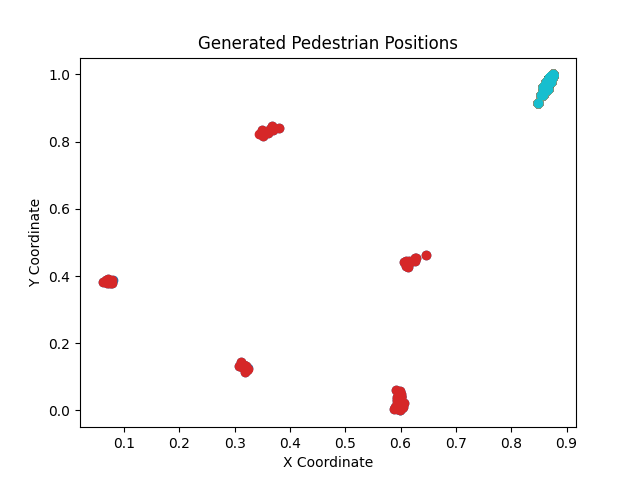
\includegraphics[width=0.8\textwidth]{Images/nomalized_epoch5.png}
    \caption{Generated samples at epoch 5 (Normalized)}
    \label{fig:epoch5_norm}
\end{figure}

\begin{figure}[H]
    \centering
    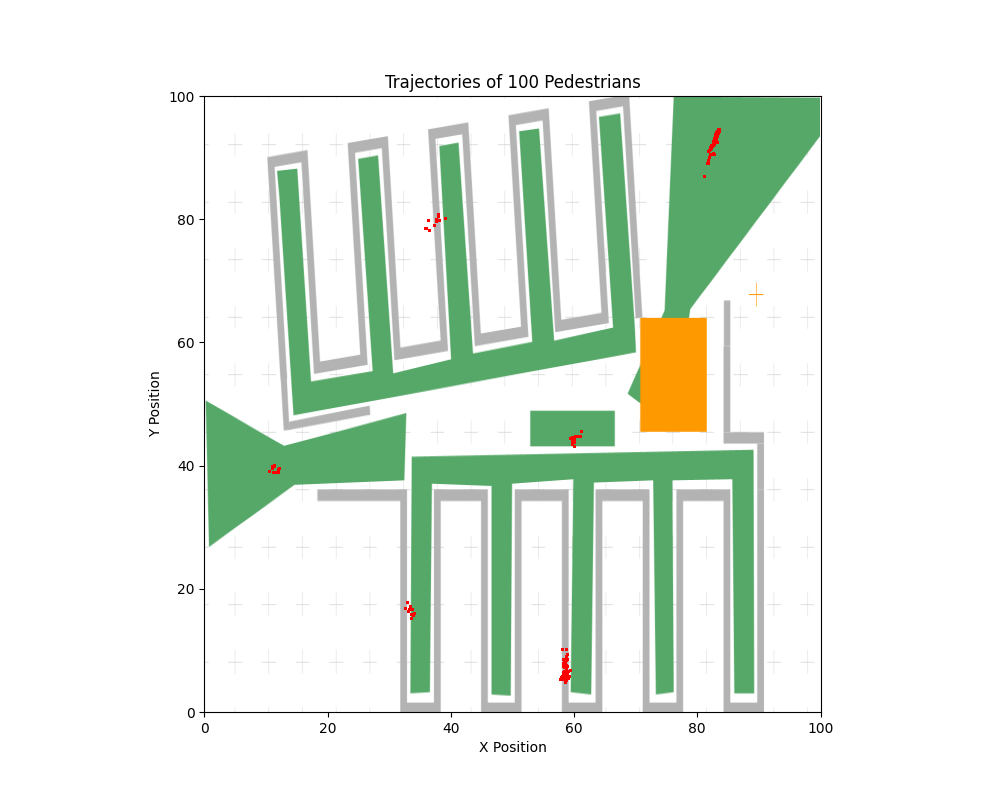
\includegraphics[width=0.8\textwidth]{Images/pedestrians_trajectories_epoch5.png}
    \caption{Generated samples at epoch 5 (Rescaled to TUM MI)}
    \label{fig:epoch5_real}
\end{figure}

\begin{figure}[H]
    \centering
    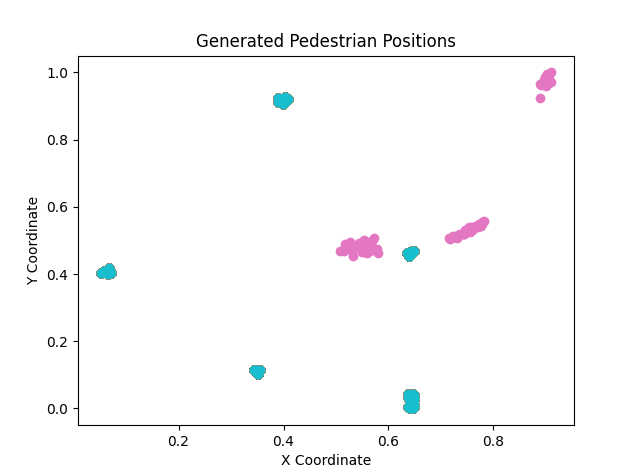
\includegraphics[width=0.8\textwidth]{Images/nomalized_epoch50.png}
    \caption{Generated samples at epoch 50 (Normalized)}
    \label{fig:epoch50_norm}
\end{figure}

\begin{figure}[H]
    \centering
    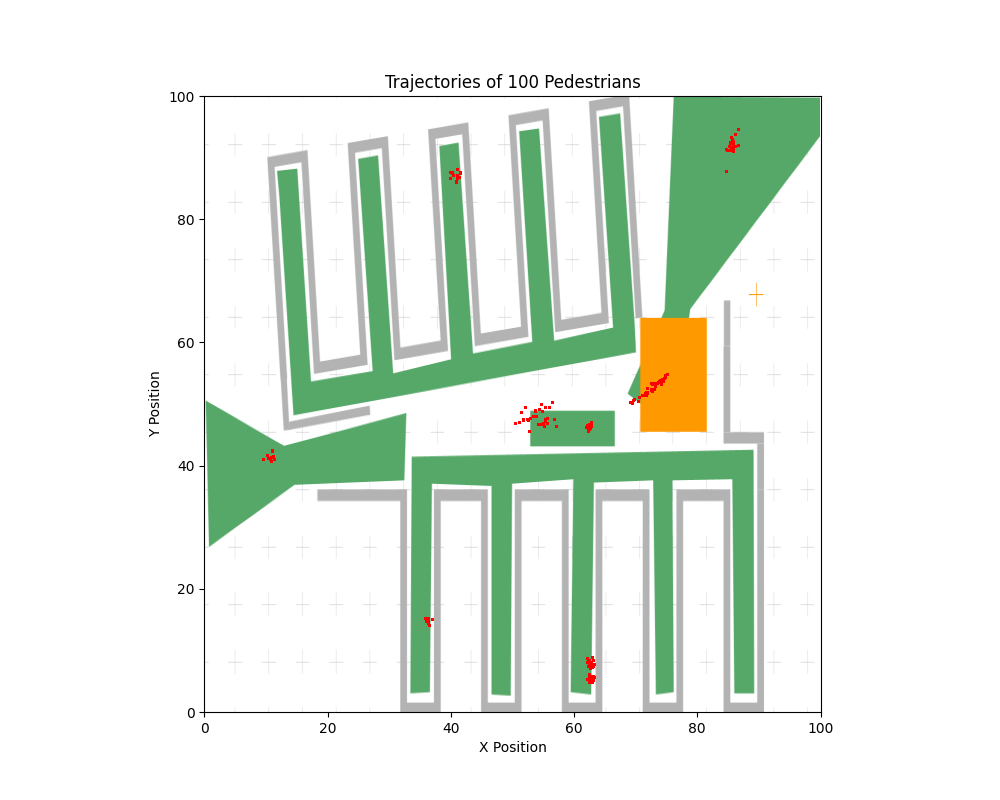
\includegraphics[width=0.8\textwidth]{Images/pedestrians_trajectories_epoch50.png}
    \caption{Generated samples at epoch 50 (Rescaled to TUM MI)}
    \label{fig:epoch50_real}
\end{figure}

\begin{figure}[h]
    \centering
    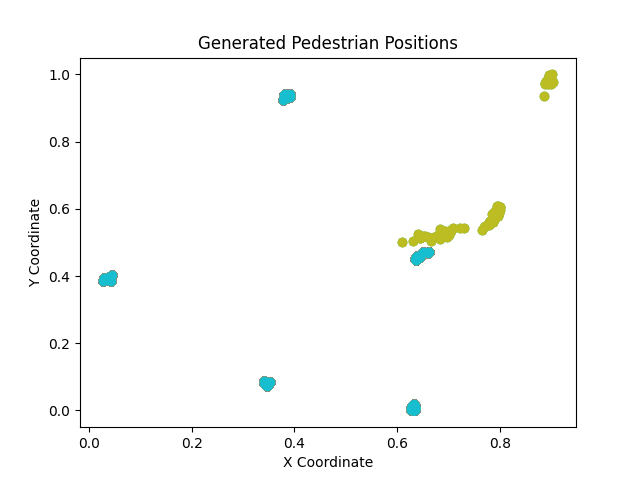
\includegraphics[width=0.8\textwidth]{Images/nomalized_epoch110.png}
    \caption{Generated samples at epoch 110 (Normalized)}
    \label{fig:epoch110_norm}
\end{figure}

\begin{figure}[H]
    \centering
    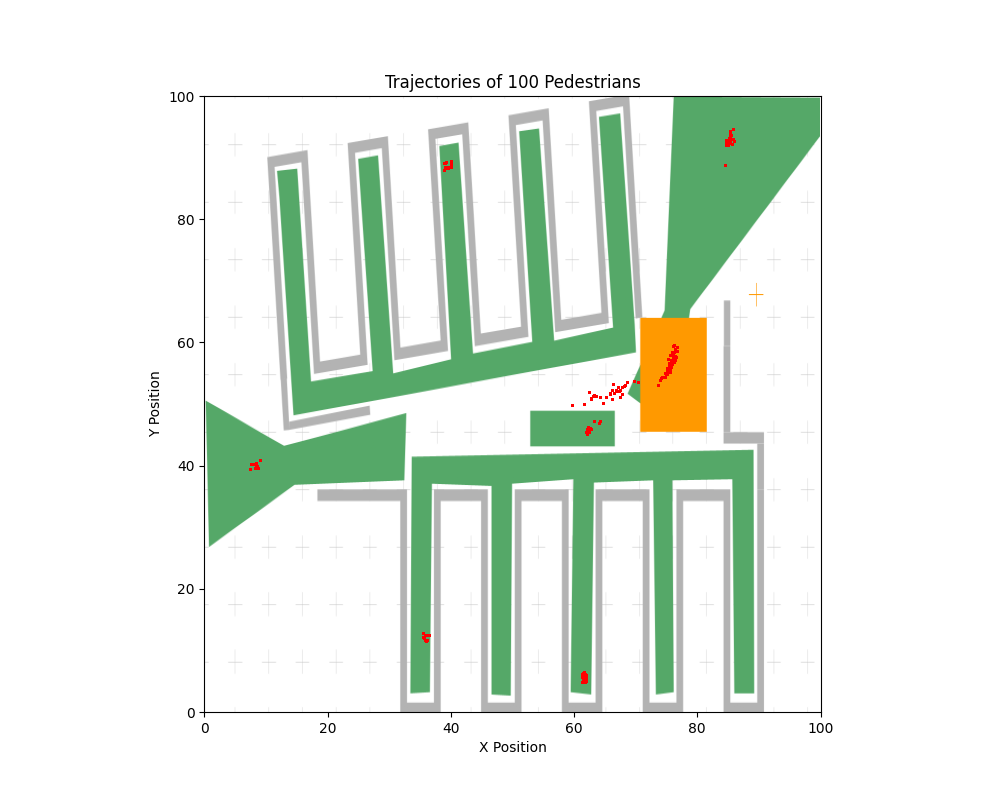
\includegraphics[width=0.8\textwidth]{Images/pedestrians_trajectories_epoch110.png}
    \caption{Generated samples at epoch 110 (Rescaled to TUM MI)}
    \label{fig:epoch110_real}
\end{figure}

\begin{figure}[H]
    \centering
    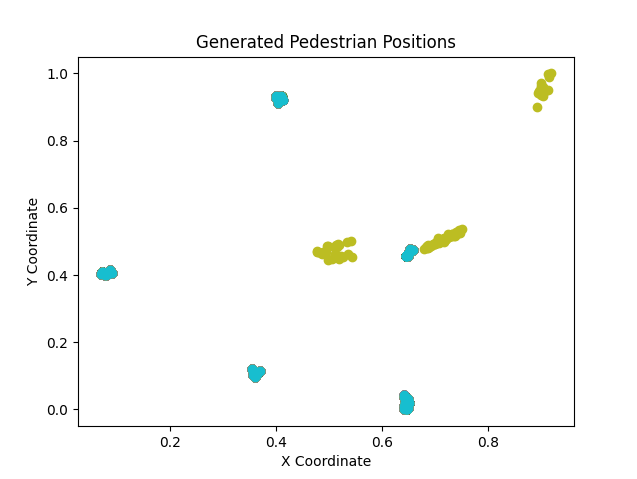
\includegraphics[width=0.8\textwidth]{Images/nomalized_epoch150.png}
    \caption{Generated samples at epoch 150 (Normalized)}
    \label{fig:epoch150_norm}
\end{figure}

\begin{figure}[H]
    \centering
    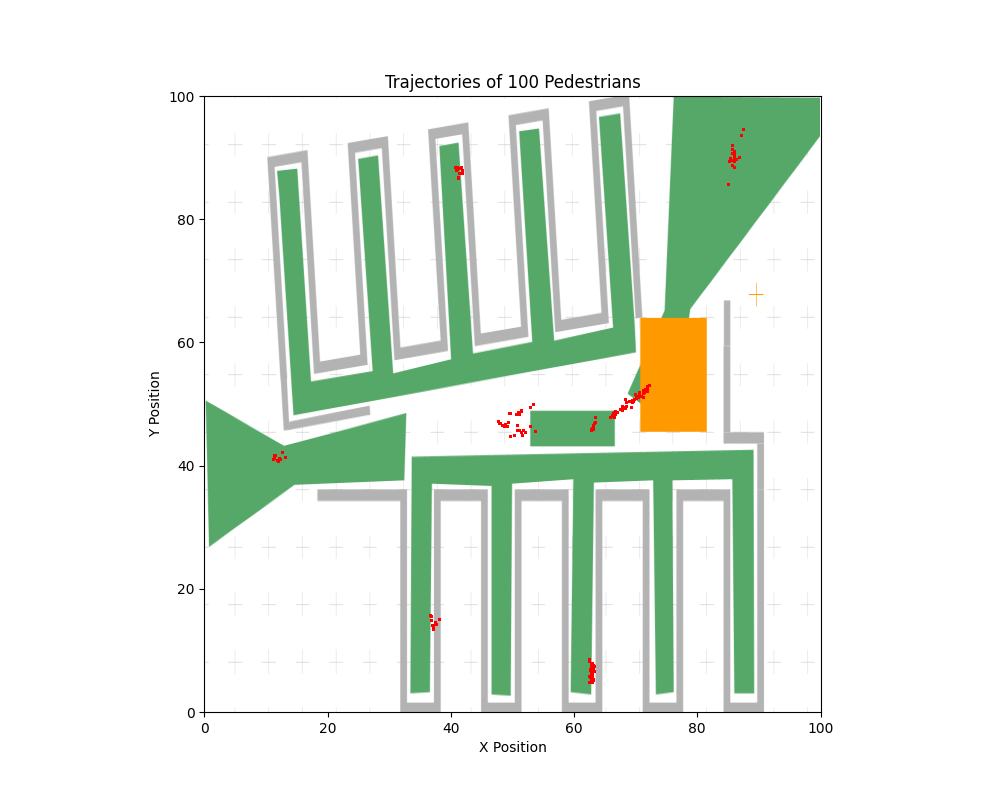
\includegraphics[width=0.8\textwidth]{Images/pedestrians_trajectories_epoch150.png}
    \caption{Generated samples at epoch 150 (Rescaled to TUM MI)}
    \label{fig:epoch150_real}
\end{figure}

\begin{figure}[H]
    \centering
    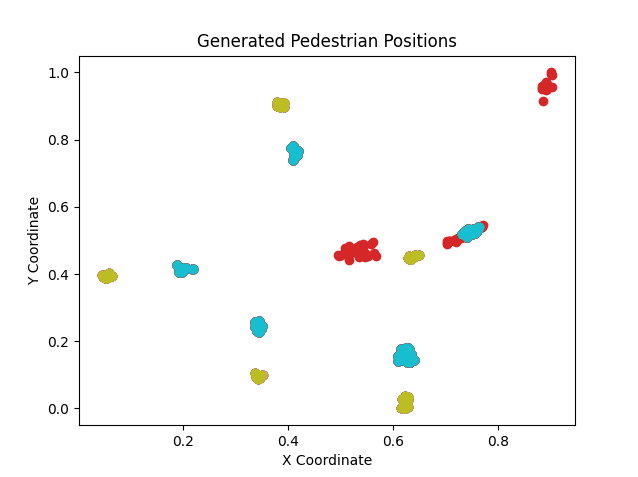
\includegraphics[width=0.8\textwidth]{Images/nomalized_epoch200.png}
    \caption{Generated samples at epoch 200 (Normalized)}
    \label{fig:epoch200_norm}
\end{figure}

\begin{figure}[H]
    \centering
    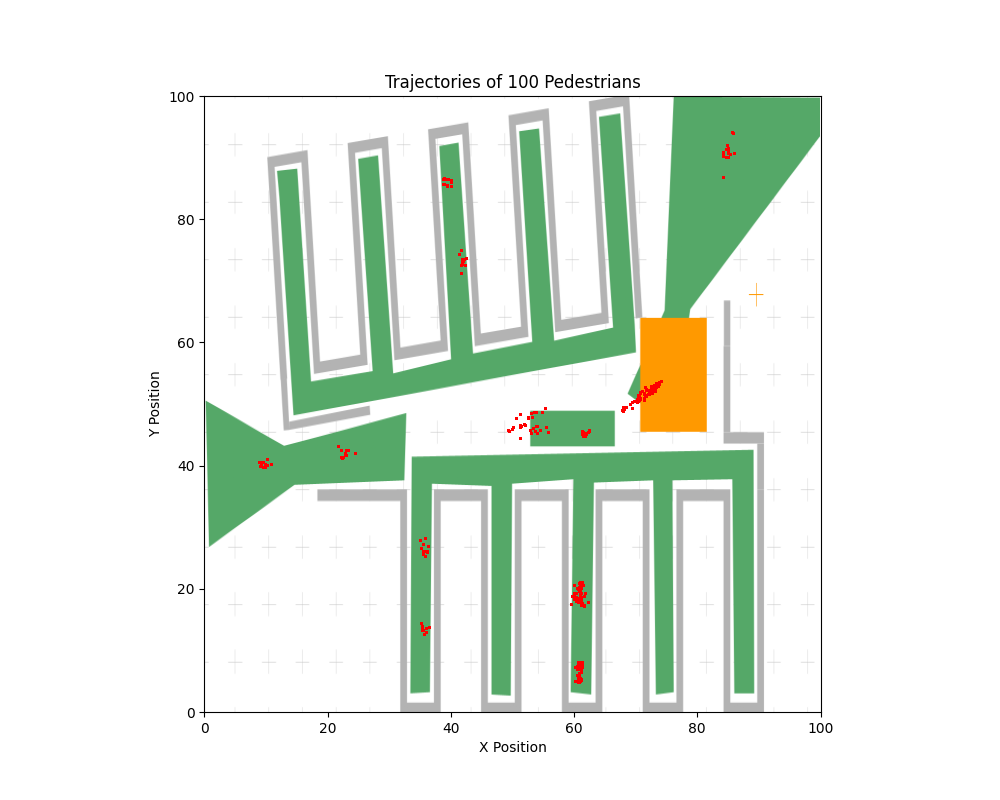
\includegraphics[width=0.8\textwidth]{Images/pedestrians_trajectories_epoch200.png}
    \caption{Generated samples at epoch 200 (Rescaled to TUM MI)}
    \label{fig:epoch200_real}
\end{figure}

\begin{figure}[H]
    \centering
    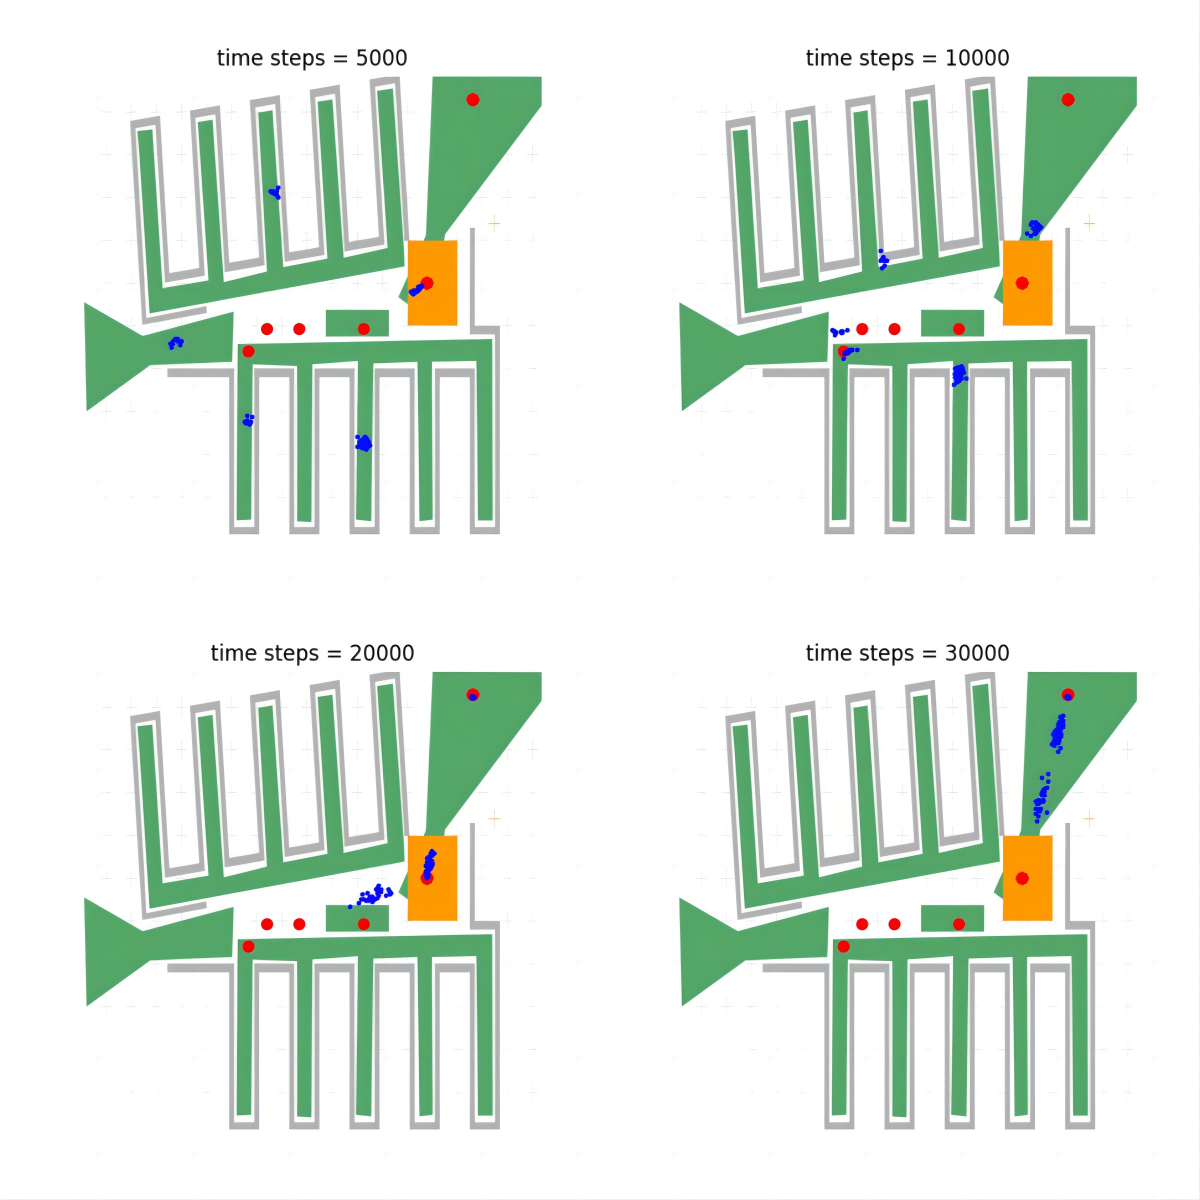
\includegraphics[width=0.8\textwidth]{Images/original_pedestrian_positions.png}
    \caption{Real data from TUM MI building}
    \label{fig:real_data}
\end{figure}
Figures \ref{fig:epoch5_norm} to \ref{fig:epoch200_real} show the visualizations of the generated pedestrian trajectories at different epochs during training. Each epoch's results include both the normalized and rescaled (to the actual scene at TUM MI building) data. Additionally, Figure \ref{fig:real_data} presents the real data for comparison.


This project successfully implements a DDPM to generate realistic pedestrian trajectories. The use of a 1D U-Net allows the model to capture both local and global patterns in the data. The training and sampling procedures ensure that the model learns the distribution of the data and can generate high-quality samples. This approach can be extended to other types of sequential data, offering a powerful tool for generative modeling.


\section*{References}

\begin{itemize}
\item Ho, J., Jain, A.,  Abbeel, P. (2020). Denoising Diffusion Probabilistic Models. In Advances in Neural Information Processing Systems (NeurIPS).
\item Sohl-Dickstein, J., Weiss, E., Maheswaranathan, N.,  Ganguli, S. (2015). Deep Unsupervised Learning using Nonequilibrium Thermodynamics. In Proceedings of the 32nd International Conference on Machine Learning (ICML).
\item Kingma, D. P.,  Welling, M. (2013). Auto-Encoding Variational Bayes. arXiv preprint arXiv:1312.6114.
\item Ling Yang, Zhilong Zhang, Yang Song, Shenda Hong, Runsheng Xu, Yue Zhao, Wentao Zhang, Bin Cui, and Ming-Hsuan Yang. 2023. Diffusion Models: A Comprehensive Survey of Methods and Applications. ACM Comput. Surv. 56, 4, Article 105 (April 2024), 39 pages. https://doi.org/10.1145/3626235
\item Mao, Weibo, et al. "Leapfrog diffusion model for stochastic trajectory prediction." Proceedings of the IEEE/CVF conference on computer vision and pattern recognition. 2023.
\item Croitoru, Florinel-Alin, et al. "Diffusion models in vision: A survey." IEEE Transactions on Pattern Analysis and Machine Intelligence 45.9 (2023): 10850-10869.
\end{itemize}

\end{document}